%!TEX program = xelatex
\documentclass[11pt,article,oneside]{memoir}
\usepackage{org-preamble-xelatex}
\DisemulatePackage{setspace}
\usepackage{setspace}
\usepackage{titling}
\setlength{\droptitle}{-12em}
% \input{vc}


\usepackage{graphicx}
% We will generate all images so they have a width \maxwidth. This means
% that they will get their normal width if they fit onto the page, but
% are scaled down if they would overflow the margins.
\makeatletter
\def\maxwidth{\ifdim\Gin@nat@width>\linewidth\linewidth
\else\Gin@nat@width\fi}
\makeatother
\let\Oldincludegraphics\includegraphics
\renewcommand{\includegraphics}[1]{\Oldincludegraphics[width=\maxwidth]{#1}}

\title{The Early Spread of Mass Media Increases the Probability of Civil War: A
Research Note}

%\author{}

\author{\Large Justin Murphy\vspace{0.05in} \newline\normalsize\emph{University of Southampton} \newline\footnotesize \url{j.murphy@soton.ac.uk}\vspace*{0.2in}\newline }

%\author{Justin Murphy (University of Southampton)}

\date{}


\begin{document}  
\setkeys{Gin}{width=1\textwidth} 	
\setromanfont[Mapping=tex-text,Numbers=OldStyle]{Georgia} 
\setsansfont[Mapping=tex-text]{Gill Sans} 
\setmonofont[Mapping=tex-text,Scale=0.8]{Consolas}
\chapterstyle{article-jmrphy}

\doublespacing


\maketitle



\vspace{-4ex}
\begin{abstract}

\noindent A recent article in \emph{International Organization} suggests that by
enhancing the soft power of states, the spread of mass media decreases
the probability of civil war onset. This research note contributes a
crucial correction to the logic of that argument (internal validity) and
demonstrates a substantively different and improved accounting of the
empirical relationship between mass media and civil war (external
validity).

\end{abstract}

\newpage


In a recent issue of \emph{International Organization}, Camber Warren
argues that mass media penetration makes civil wars less likely because
mass media enhances state strength and therefore deters potential
insurgents. Warren argues that the well-known cases in which mass media
are often believed to have facilitated civil war, such as Yugoslavia and
Rwanda in the early 1990s, are misleading examples selected on the
dependent variable. Indeed, his account argues that these are cases of
low mass media penetration (Warren 2014, 124) and are better understood
as examples of how weak mass media systems increase the probability of
civil war.

While Warren's article is an original and important study which presents
numerous and convincing robustness checks for its main conclusion, the
overall argument suffers from a crucial flaw. If

If the level of mass media \emph{in general} decreases the probability
of civil war, as Warren argues, then the complete absence of mass media
should be associated with an even lower probability of civil war than
low levels of mass media. Further, the very lowest levels of mass media
should be associated with a higher probability of civil war than
slightly higher levels of mass media. However, empirically, neither of
these implications are true. First, the contemporary era in which mass
media has most proliferated around the globe has seen more civil wars
than the period prior to the proliferation of mass media, a stylized
fact strikingly inconsistent with but unacknowledged by Warren's
argument. Second, while the probability of observing civil war
consistently approaches zero after a mass media density of roughly 35\%
consistently approaches zero (with not a single civil war in any country
with more than a mass media density of 145\%), the very lowest levels of
observed mass media are more positively associated with civil war than
countries with slightly more mass media.{[}\^{} Footnote about cutpoints
and robustness{]}

then a low level of mass media should be associated with a higher
probability of civil war than the absence of mass media.

Warren fails to consider the possibility

I argue that the \emph{the introduction and early growth of mass media}
increases the probability of civil war. While Warren demonstrates a
theoretically and empirically robust negative relationship between
levels of mass media and the probability of civil war onset, he

I provide an alternative characterization which extends \emph{low levels
of mass media make civil war more likely than the absence of mass
media,} but that beyond a certain threshold mass media make civil war
less likely. In other words, Warren sets up a straw man to characterize
the well-known cases of media and civil war, representing that
hypothesis to mean ``the more media, the more likely civil war''. But
perhaps the most theoretically sensible version of that hypothesis is
that early growth of mass media makes civil wars more likely?

I argue that this is precisely BECAUSE after about 35\% of media density
civil war against the state is no longer possible. Because state control
with mass media is so much more durable than without the presence of
mass media, once mass media is introduced into the national political
arena, it increases incentives for insurgencies. People who previously
believed in slow and steady non-violent struggle against the state
realize that once the country is thoroughly penetrated by mass media,
non-violent struggles to fundamentally challenge the state will become
nearly impossible. This shifts some portion of the non-violent
challengers to become violent rebels.

If Warren's argument is correct, it implies incentives for civil war
from the early spread of mass media.

\begin{figure}[htbp]
\centering
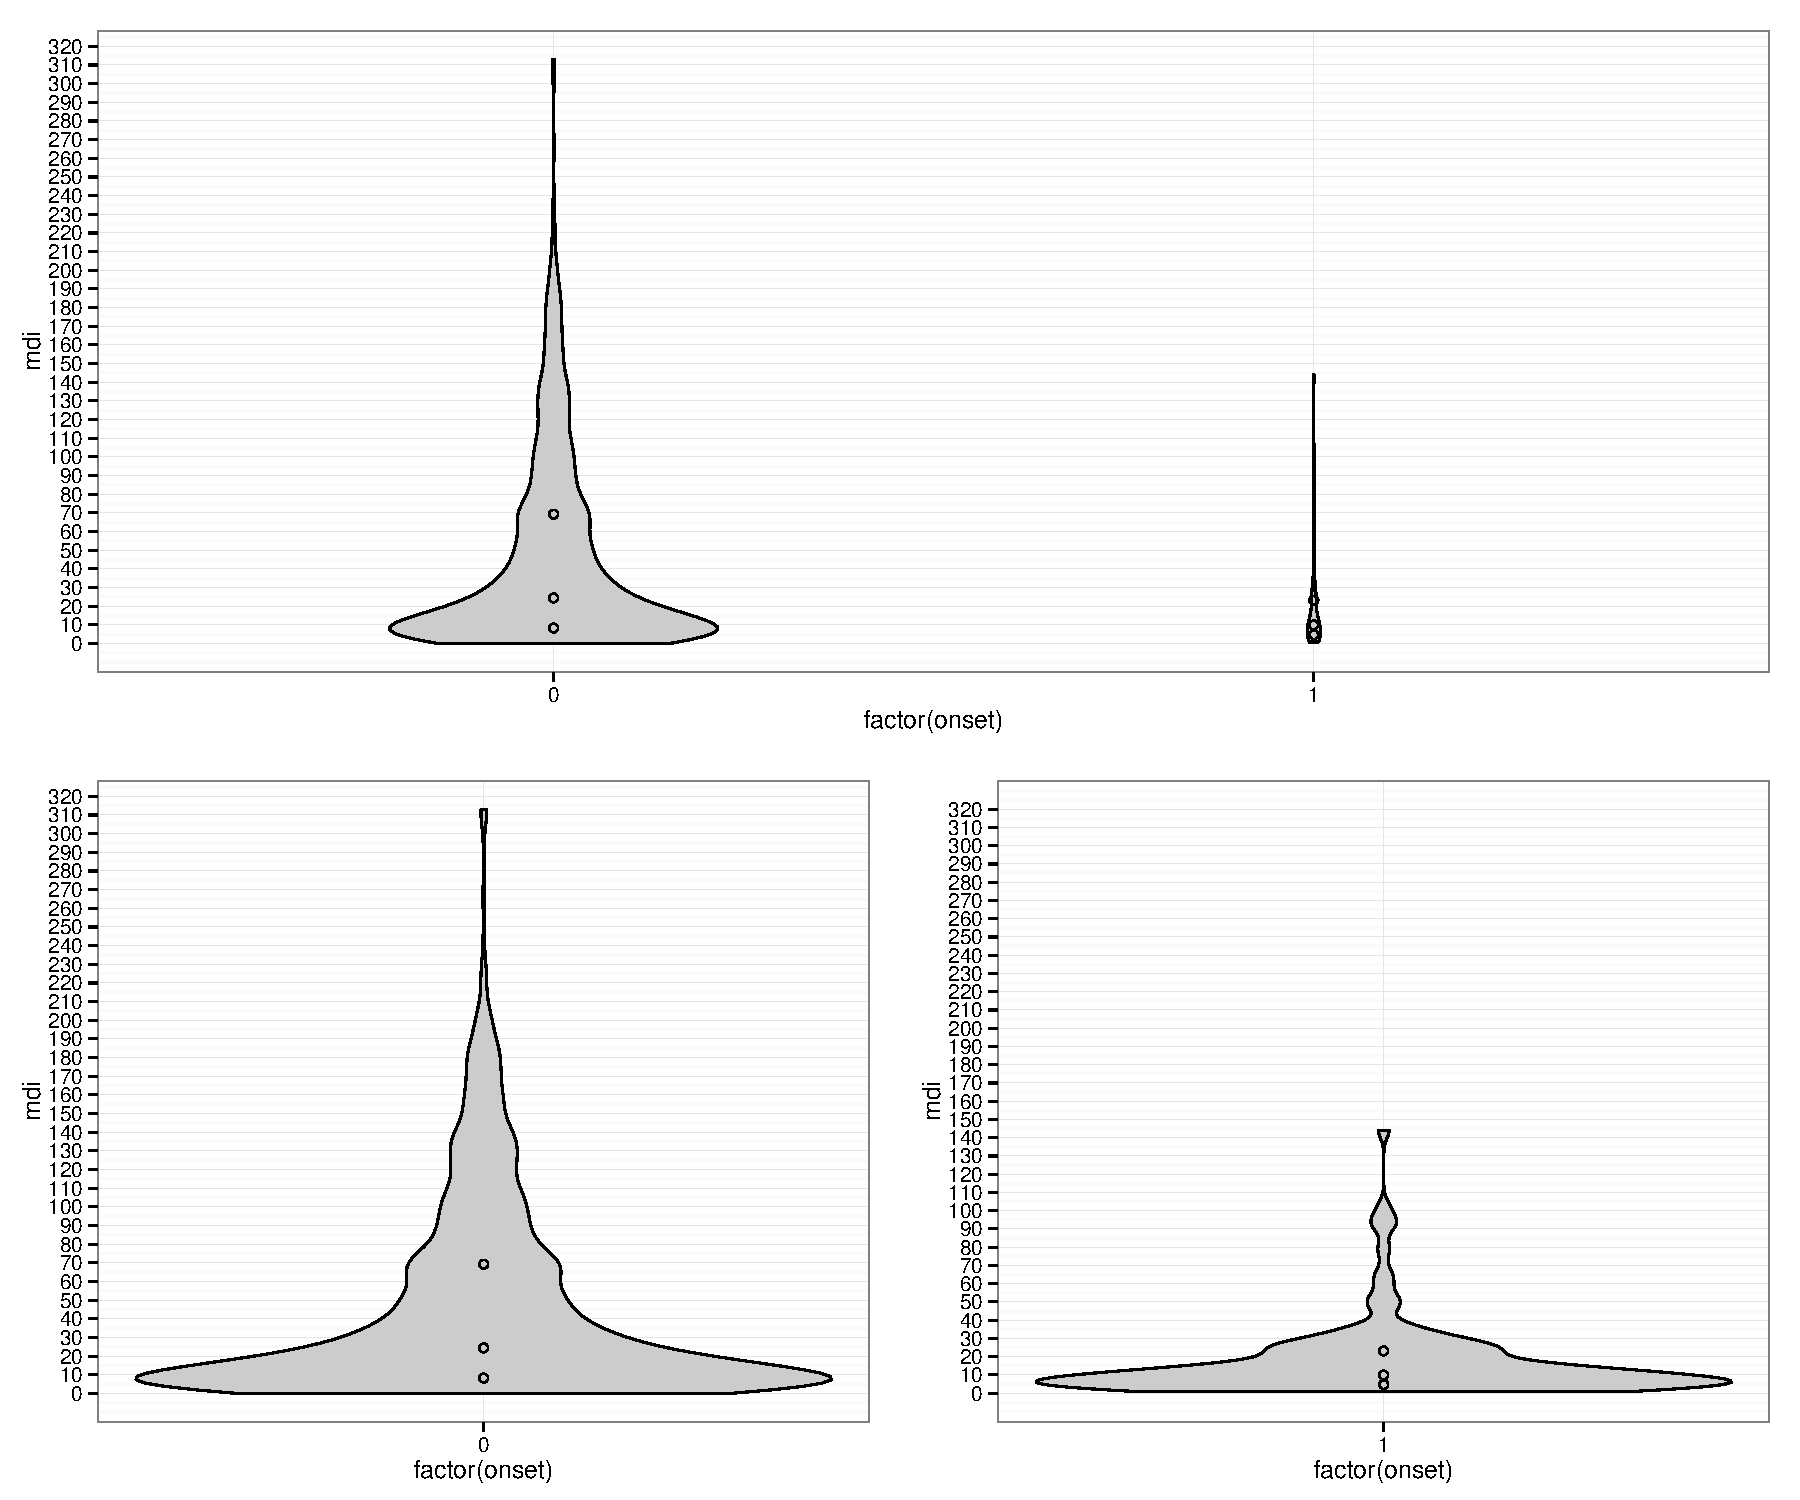
\includegraphics{figure/violinplot.pdf}
\caption{Violin plot of media density for all civil war onsets}
\end{figure}

\begin{table}[!htbp] \centering 
  \caption{Early Growth of Media Density Compared to Media Density in General} 
  \label{} 
\footnotesize 
\begin{tabular}{@{\extracolsep{5pt}}lccc} 
\\[-1.8ex]\hline \\[-1.8ex] 
\\[-1.8ex] & \multicolumn{3}{c}{onset} \\ 
\\[-1.8ex] & (1) & (2) & (3)\\ 
\hline \\[-1.8ex] 
 mdi & $-$0.03$^{***}$ &  &  \\ 
  & (0.01) &  &  \\ 
  ld.mdi &  & 0.51$^{**}$ &  \\ 
  &  & (0.26) &  \\ 
  ld.news &  &  & 1.44$^{*}$ \\ 
  &  &  & (0.75) \\ 
  ld.radio &  &  & 0.27 \\ 
  &  &  & (0.31) \\ 
  ld.tv &  &  & 2.10$^{*}$ \\ 
  &  &  & (1.22) \\ 
  lgdpl & $-$0.04 & $-$0.49 & $-$0.49 \\ 
  & (0.17) & (0.32) & (0.31) \\ 
  larea & $-$0.09 & 0.01 & 0.001 \\ 
  & (0.09) & (0.15) & (0.15) \\ 
  lmtn & 0.11$^{*}$ & 0.12 & 0.11 \\ 
  & (0.06) & (0.09) & (0.09) \\ 
  lpopl & 0.27$^{***}$ & 0.28$^{**}$ & 0.28$^{**}$ \\ 
  & (0.09) & (0.13) & (0.13) \\ 
  oil2l & 0.76$^{***}$ & 1.12$^{**}$ & 1.16$^{**}$ \\ 
  & (0.28) & (0.47) & (0.48) \\ 
  deml & 0.18$^{**}$ & 0.24$^{*}$ & 0.23$^{*}$ \\ 
  & (0.08) & (0.12) & (0.12) \\ 
  deml2 & $-$0.01$^{**}$ & $-$0.01 & $-$0.01 \\ 
  & (0.003) & (0.01) & (0.01) \\ 
  ethfracl & 0.20 & $-$0.73 & $-$0.59 \\ 
  & (0.37) & (0.54) & (0.55) \\ 
  relfracl & 1.38$^{***}$ & 1.27 & 1.38$^{*}$ \\ 
  & (0.52) & (0.79) & (0.79) \\ 
  pcyrs & $-$0.06 & $-$0.10 & $-$0.10 \\ 
  & (0.09) & (0.12) & (0.12) \\ 
  spline1 & $-$0.0001 & $-$0.001 & $-$0.002 \\ 
  & (0.002) & (0.003) & (0.003) \\ 
  spline2 & $-$0.0002 & 0.0003 & 0.0004 \\ 
  & (0.001) & (0.001) & (0.001) \\ 
  spline3 & 0.0001 & 0.0000 & $-$0.0000 \\ 
  & (0.0002) & (0.0003) & (0.0003) \\ 
  Constant & $-$8.35$^{***}$ & $-$9.59$^{***}$ & $-$9.65$^{***}$ \\ 
  & (1.18) & (1.77) & (1.80) \\ 
 N & 5,899 & 1,672 & 1,672 \\ 
Log Likelihood & $-$527.50 & $-$219.80 & $-$218.40 \\ 
AIC & 1,085.00 & 469.60 & 470.70 \\ 
\hline \\[-1.8ex] 
\multicolumn{4}{l}{$^{*}$p $<$ .1; $^{**}$p $<$ .05; $^{***}$p $<$ .01} \\ 
\end{tabular} 
\end{table}

\begin{figure}[htbp]
\centering
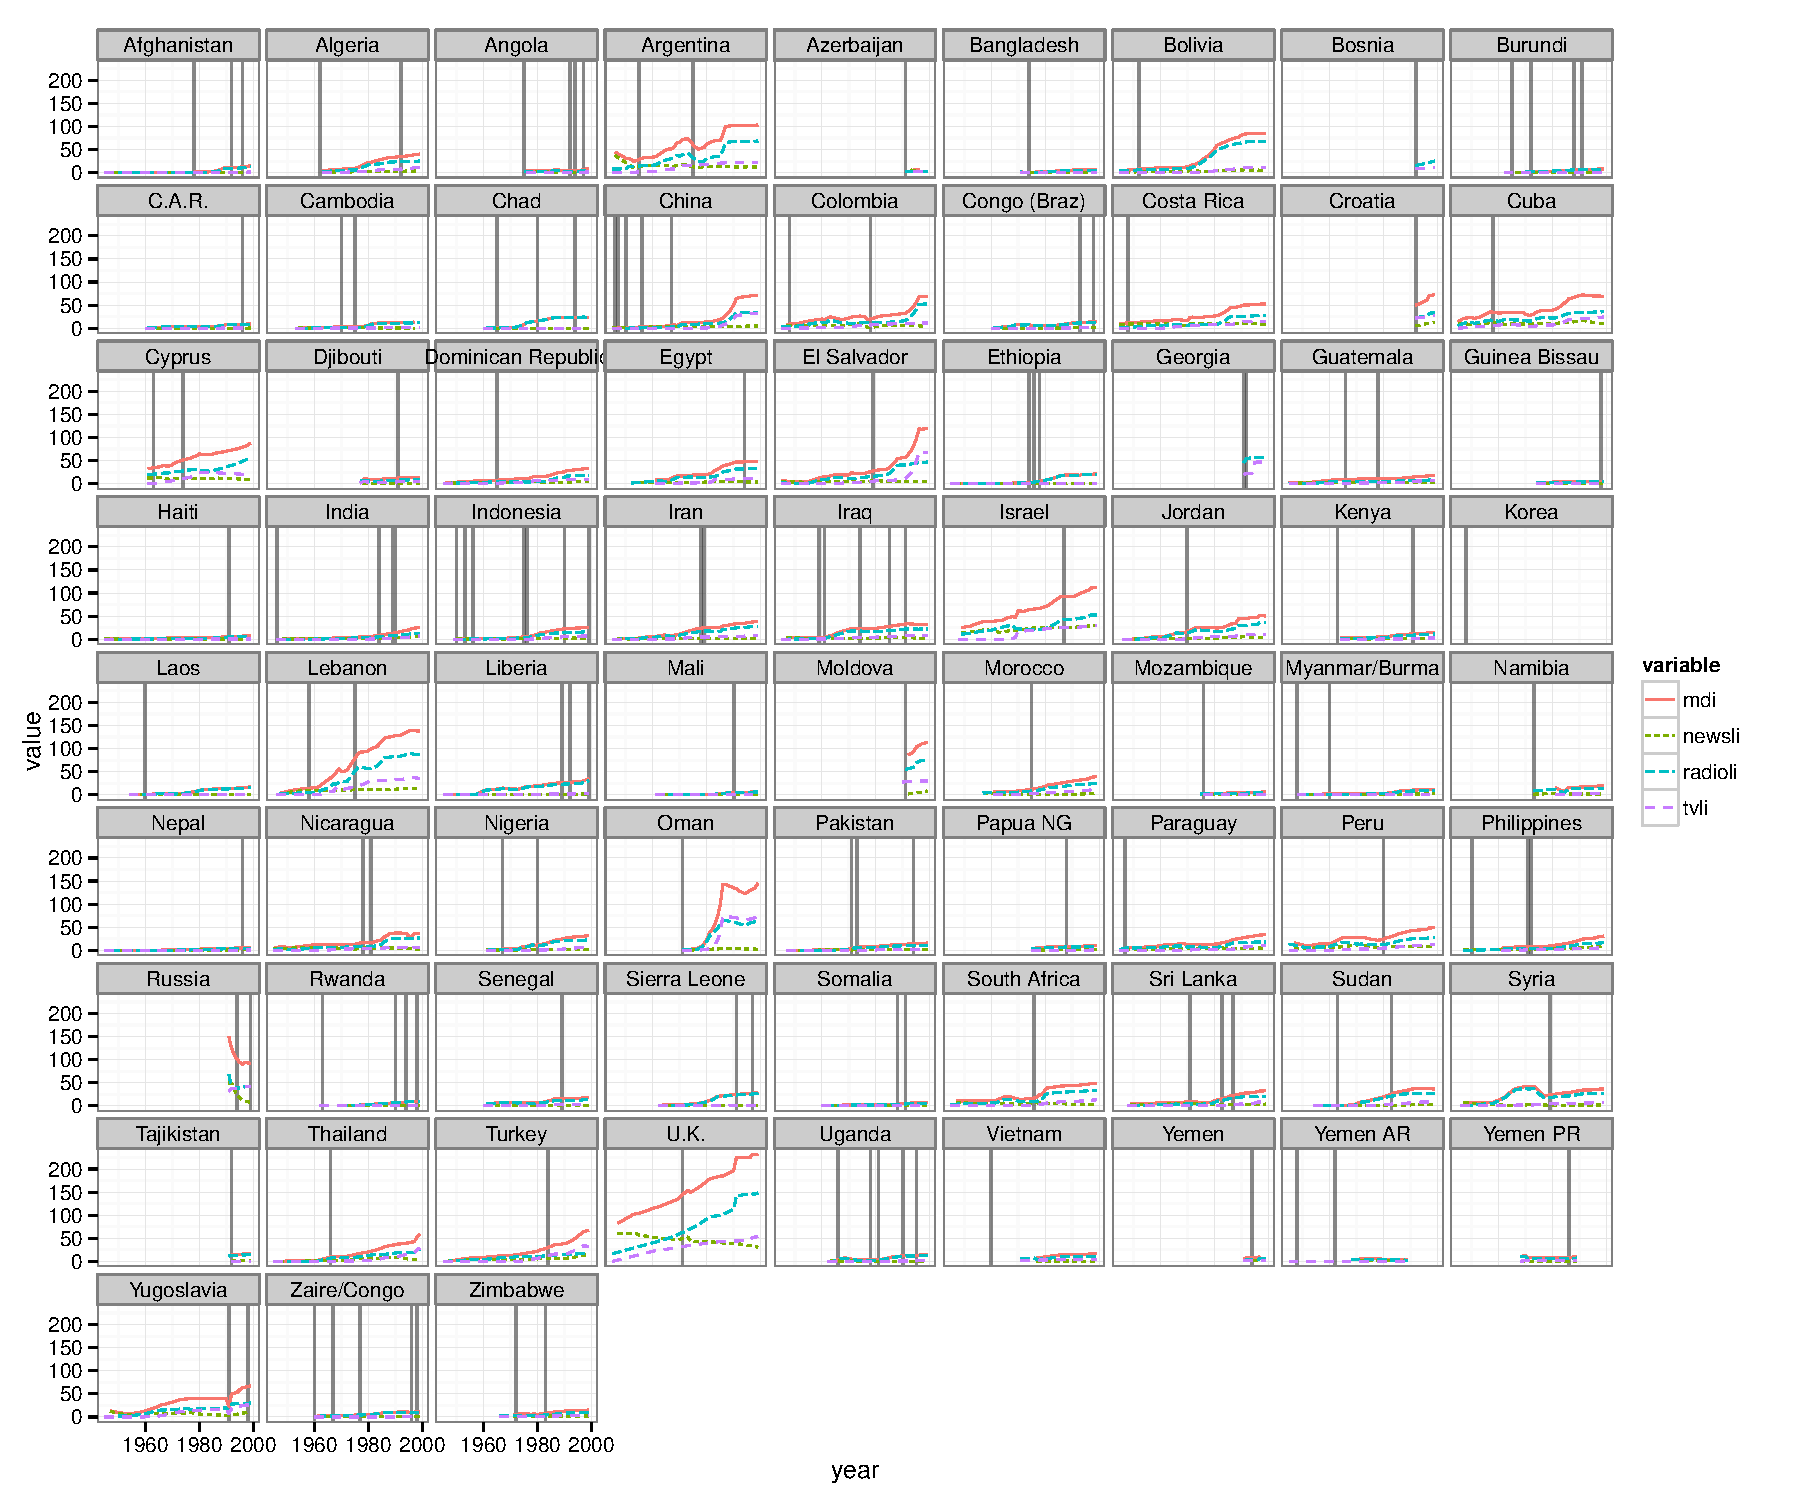
\includegraphics{figure/full_panel_plot.pdf}
\caption{Disaggregated media density and all civil war onsets over time,
by country}
\end{figure}

Warren, T Camber. 2014. ``Not by the Sword Alone: Soft Power, Mass
Media, and the Production of State Sovereignty.'' \emph{International
Organization} 68(01): 111--41.
\url{http://www.journals.cambridge.org/abstract_S0020818313000350}.


\end{document}